\documentclass[../main.tex]{subfiles}
\graphicspath{{figures/}{../figures/}}

\begin{document}
% \todo[color=green!30]{完成问题二模型的求解(sections/q2\_solution)}

我们利用模拟退火算法求解上述单目标优化模型。
核心思路是:通过模拟物理退火过程的随机搜索与概率接受机制,在决策变量的可行域内寻找使有效遮蔽时间$\Delta t$最大化的最优解。具体步骤如下:

\noindent \textbf{步骤1$\,\,$设定初始参数和离散化时间轴}

根据题目要求和经验,设定干扰弹发射角度、速度及投放时间等初始参数。将导弹飞行时间段划分为细小的时间步长,便于逐点判断遮蔽状态。

\noindent \textbf{步骤2 $\,\,$遍历时间点并判断遮蔽}

对每个时间点,计算干扰弹位置,结合导弹与目标几何关系,根据模型分析中的判断条件,判断各时间点是否满足有效遮蔽条件。收集所有满足遮蔽条件的时间点,累加得到总有效遮蔽时间。

\noindent \textbf{步骤3 $\,\,$应用模拟退火算法}

 以总遮蔽时间作为目标函数值,供优化算法调用。
 通过迭代生成新参数解,依据目标函数值变化和Metropolis准则接受或拒绝新解。\\
    Metropolis准则:以一定的概率接受一个新状态,即使这个新状态的能量(或目标函数值)比当前状态更低。这有助于算法跳出局部最优解,探索更广阔的状态空间。本代码中选择的比较值是$\exp \left( \frac{\Delta S}{T} \right)$ ,其中$\Delta S$为新旧有效时间之差,$T$为该次循环的温度。当新解更大时,选用新解;新解更小时,以$\exp \left( \frac{\Delta S}{T} \right)$的概率选用新解。

\noindent \textbf{步骤4 $\,\,$逐步优化并收敛}

随着迭代进行,不断更新最优参数组合,使有效遮蔽时间逐渐增加,最终趋于稳定最优值。
\begin{figure}[H]
\centering
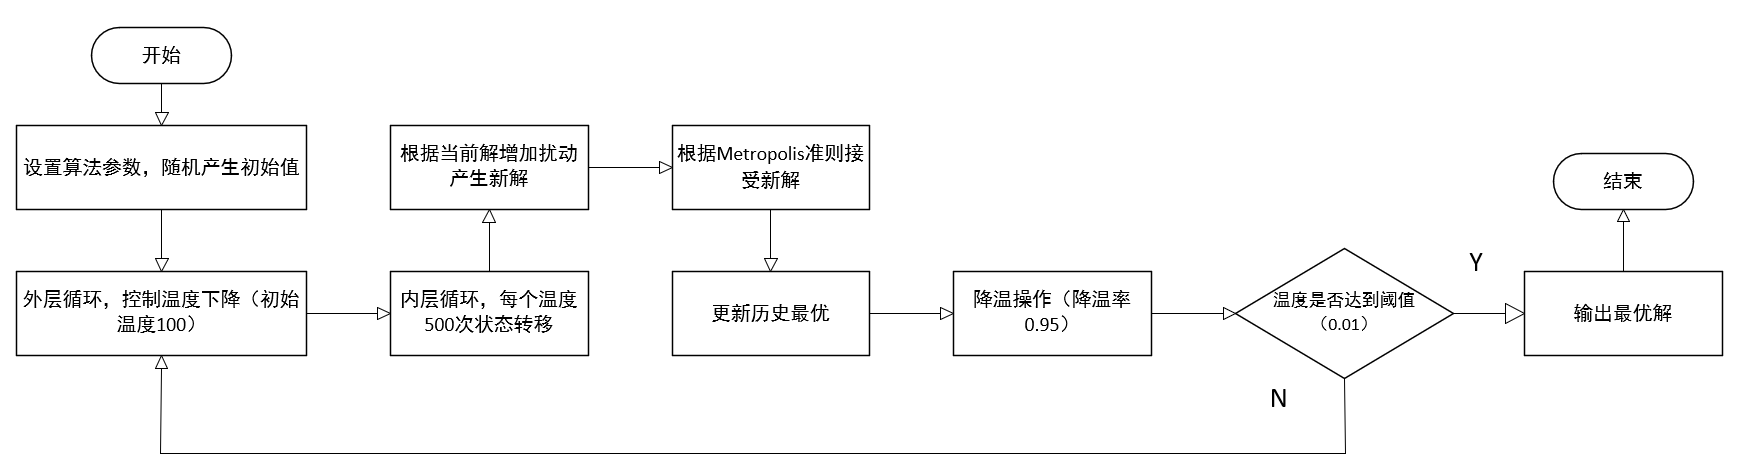
\includegraphics[scale=0.35]{问题二模型求解流程图.png}
\caption{问题二模型求解流程图}
\label{图2}
\end{figure}

按照上述算法思路,利用Python求解得当$FY1$的飞行方向与$x$轴正方向的夹角$\alpha$为3.13rad(逆时针为正),飞行速度为109.78m/s,烟雾弹投放位置为
\begin{align}
(17722.061437,0.903555,1800.000000),
\end{align}
烟雾弹起爆位置为
\begin{align}
(17335.661803,5.383153,1739.287040)
\end{align}
时,\textbf{遮蔽时间最长为4.602140秒}。







\end{document}